\subsection{Aufgabe 4 und 5}
In diesem Versuch untersuchen wir die Abh�ngigkeit der Amplitude von D�mpfung und Anregefrequenz. Das Drehpendel mit der aus den vorherigen Versuchen bekannten Eigenschwingfrequenz wird mit Hilfe des Exzenters zu einer erzwungenen Schwingung angeregt. Nach dem Einschwingen wird jeweils die Amplitude gemessen, und gegen die Anregefrequenz aufgetragen. Dies f�hrt man f�r zwei verschiedene D�mpfungen durch. Hierzu wird die Wirbelstrombremse mit verschiedenen Stromst�rken betrieben.\\
Zur Auswertung muss die Drehfrequenz des Motors bekannt sein. Diese ist in dem von uns betrachteten Spannungsbereich linear zur Motorspannung. Daher bestimmen wir zun�chst den Zusammenhang zwischen Spannung und Freqeunz aus Messungen bei verschiedenen Spannungen.
\begin{figure}[h]
	\centering
	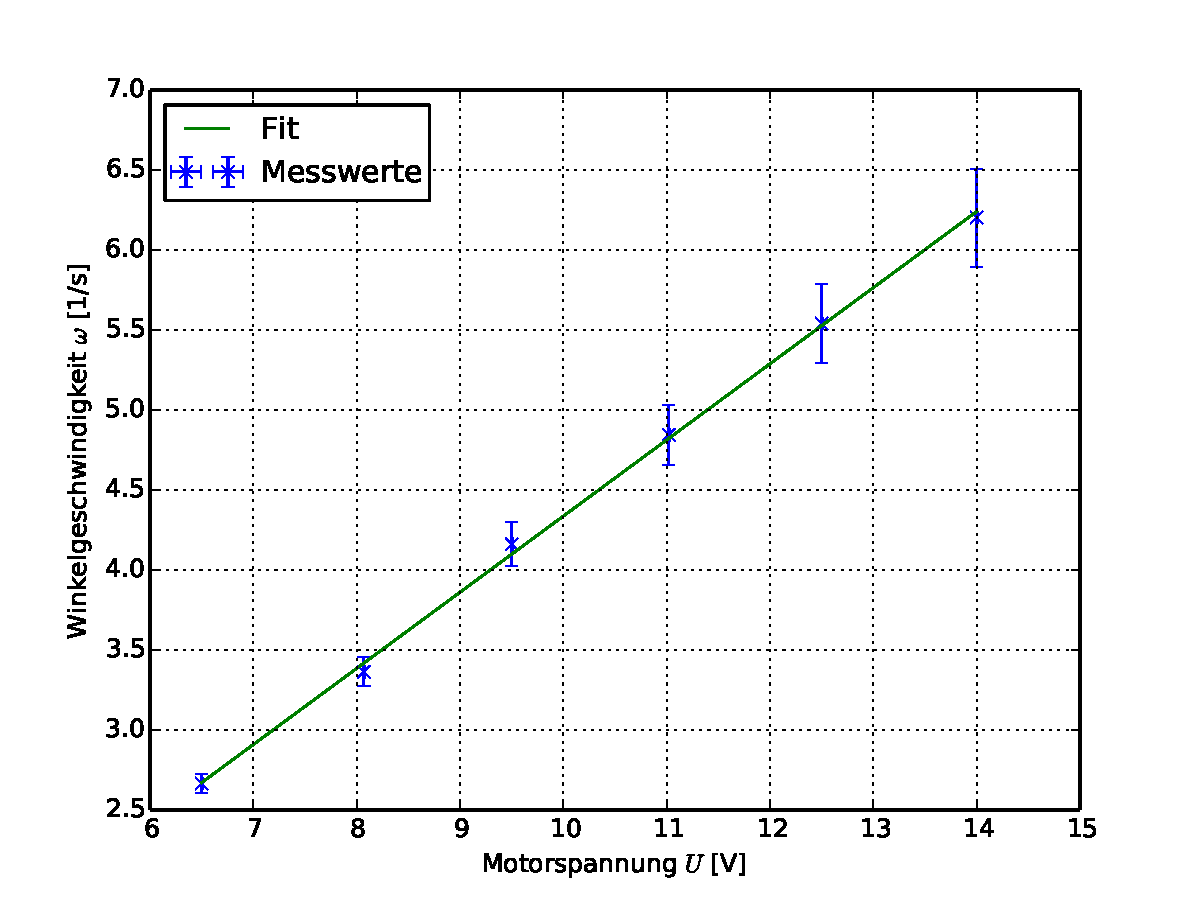
\includegraphics[width=\linewidth]{diagramme/eichkurve.pdf}
	\caption[Eichkurve]{Gemessene Spannungen gegen Winkelgeschwindigkeit aufgetragen}
	\label{fig:Eichkurve}
\end{figure}\\
Aus dem Fit der Messwerte erh�lt man unter Minimierung der Abstandsquadrate die Steigung $ (0{,}4759 \pm 0{,}0275)~\si{\per\second\per\volt} $ und den Achsenabschnitt $ (-0{,}4220 \pm 0{,}0804) \si{\per\second} $. Somit kann man durch 
\begin{equation*}
	\omega = \SI{0.4759}{\per\second\per\volt} U - \SI{-0.4220}{\per\second} \qquad \text{(+ber�cksichtigung der Fehler)}
\end{equation*}
$ U $ in $ \omega $ umrechnen. Tr�gt man $ \omega $ gegen die Amplitude $ \varphi $ auf, so ergibt sich Abbildung \ref{fig:Erzwungen}.
\begin{figure}[h]
	\centering
	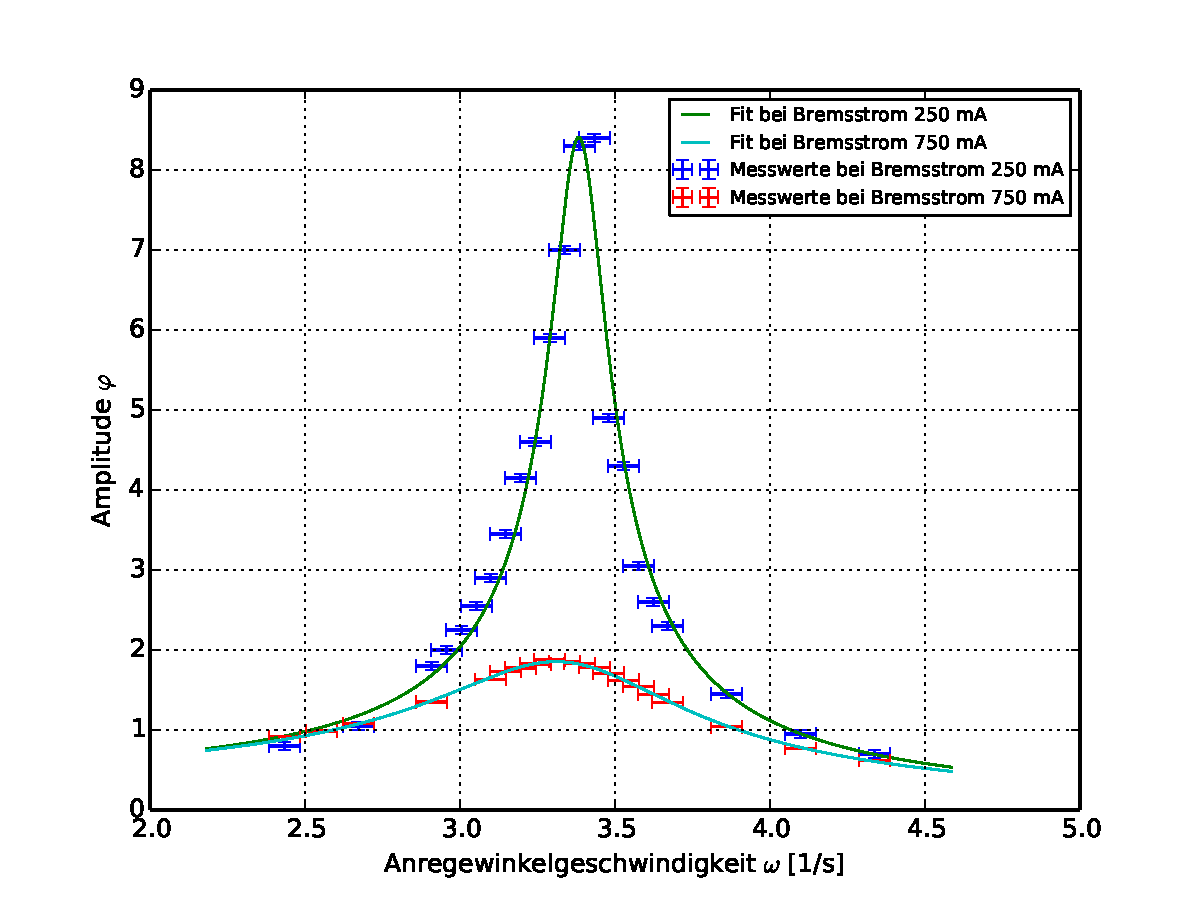
\includegraphics[width=\linewidth]{diagramme/5).pdf}
	\caption[Amplitudenfunktion]{Amplitude gegen Anregefrequenz aufgetragen}
	\label{fig:Erzwungen}
\end{figure}\\
Der Fit wurde mit der aus der Theorie bekannten Funktion f�r die Amplitude einer erzwungenen Schwingung erstellt. Der Fit unter Minimierung der Fehlerquadrate liefert als einen der Parameter die D�mpfung. Somit ist die D�mpfung jeweils:\\
\begin{tabular}{r@{: }l}
$ \SI{250}{\milli\ampere} $ & $ (0{,}090 \pm 0{,}010)~\si{\per\second} $ \\
$ \SI{750}{\milli\ampere} $ & $ (0{,}407 \pm 0{,}010)~\si{\per\second} $
\end{tabular}
\subsubsection{Diskussion}
Die theoretisch ermittelten Zusammenh�nge decken sich gut mit unseren Beobachtungen. Insbesondere an Abbildung \ref{fig:Erzwungen} ist zu sehen, dass sich eine Ausgleichskurve entsprechend der Theorie fitten l�sst, die ziemlich genau durch die Messwerte geht. Jedoch war wie auch bei vorherigen Versuchen eine die gr��te Quelle der Unsicherheit die Zeitnahme mit der Stoppuhr. Zudem stellten wir beim Erstellen der Eichkurve fest, dass sich der Motor schon knapp unterhalb der betrachteten Spannungen nicht mehr linear bez�glich der Frequenzen verh�lt. Damit erkl�rt sich unter anderem auch, dass die Ausgleichsgerade keine Ursprungsgerade ist.